\subsection{Fair CV}
One of the main goals of the Disciplina platform is to provide a way for the Students to easily prove their educational records. We propose to duplicate the records in the Student's \textit{digital CV.} This CV contains all the records that the parties have generated during the Student's educational process along with the validity proofs of that data (see figure \ref{fig:cv}).

\begin{figure}[ht]
\centering
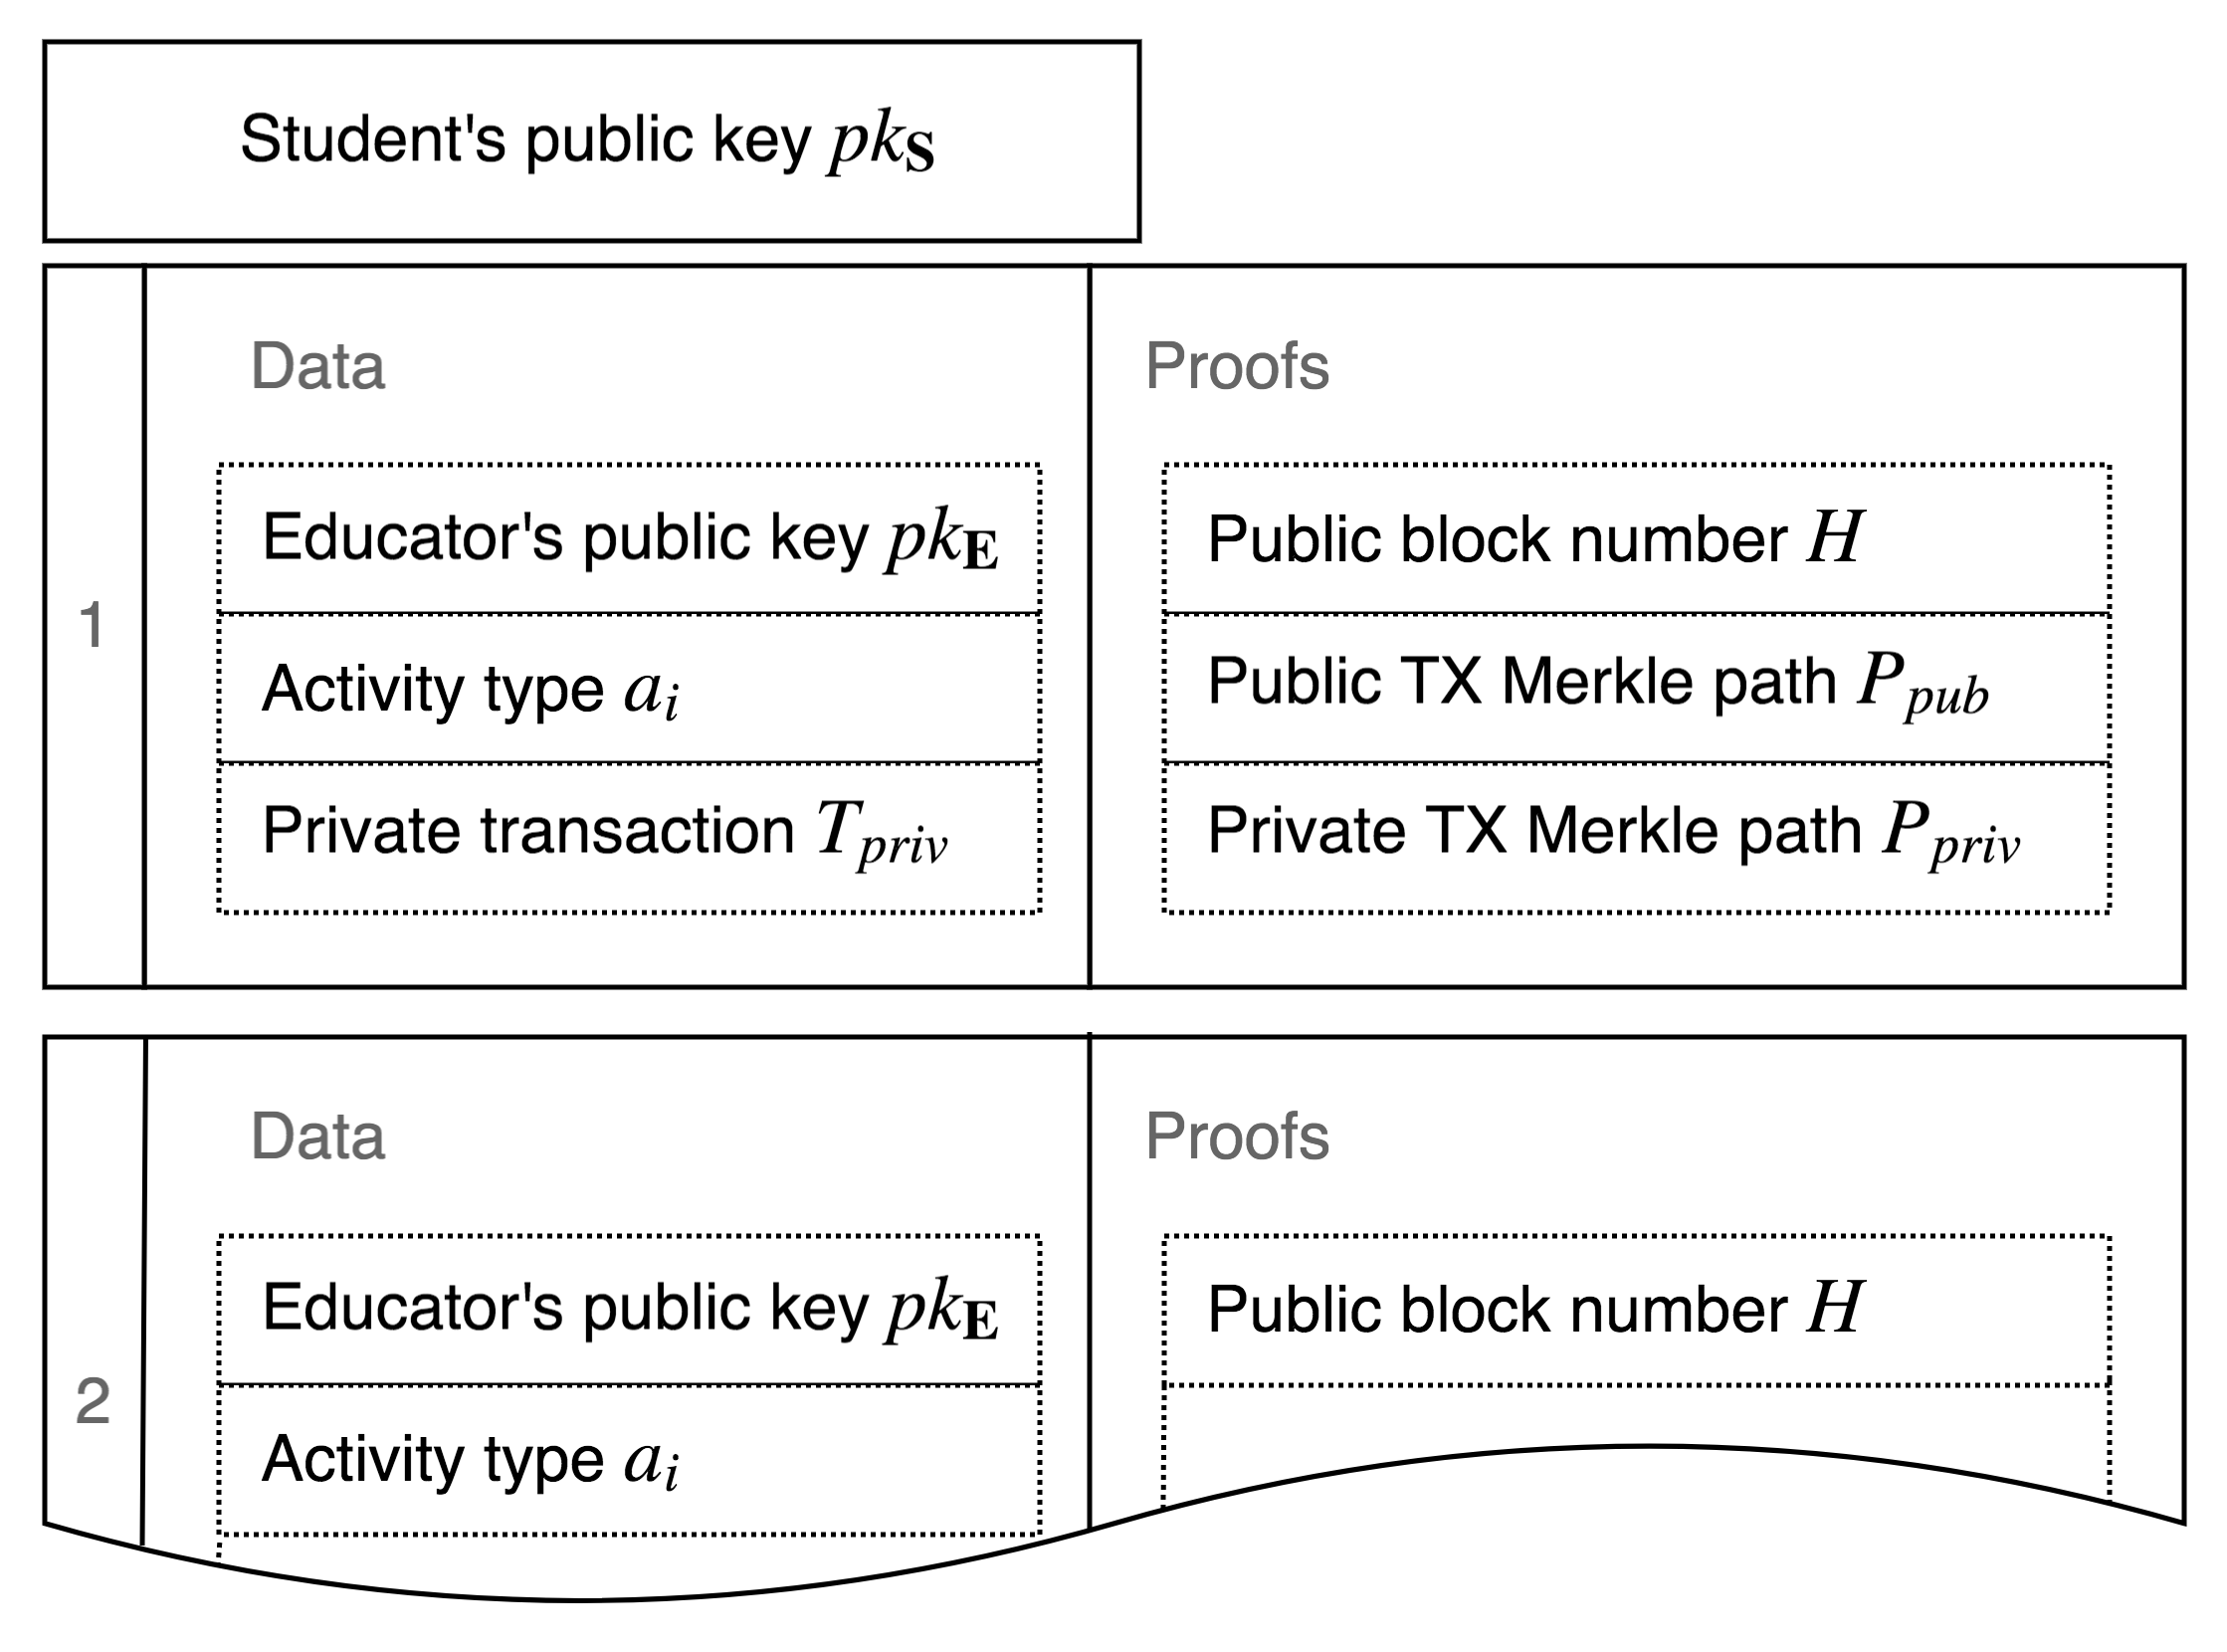
\includegraphics[width=0.8\textwidth]{cv}
\caption{Student's authenticated CV}
\label{fig:cv}
\end{figure}

In order to prove that some transaction actually occurred in some private block of the concrete Educator, the student has to provide the cryptographic proofs along with the actual data. The cryptographic proof of the inclusion of an element in an authenticated data structure is generally a path of hashes. Let us denote the path of the element $e$ in some authenticated data structure $X$ as $\Path(e, X)$. Thus, the Student has to  provide the following data:
\begin{itemize}
  \item The Student's and the Educator's public keys $\PubKey{S}$ and $\PubKey{E}$.
  \item The course $a_i$ and the a private transaction $T_{priv}$ with the score.
  \item The Merkle path of the transaction in the journal: $P_{priv} = \Path(T_{priv}, M_{priv})$, where $M_{priv}$ is a Merkle tree of the transactions in the private block.
  \item The public block number $H$ and the Merkle path of the transaction $T_{pub}$ that pushed the private block into the public chain: $P_{pub} = \Path(T_{pub}, M_{pub})$, where $M_{pub}$ is a Merkle tree of the transactions in the block $H$.
\end{itemize}

Having this data one can prove the occurrence of a certain transaction in one of the Educator's private blocks without the need to request any data from the Educator during the validation process. Thus, any party can check the validity of the Student's CV for free if the Student wishes to disclose it.

Let $\rho(e, P)$ be the function that substitutes the element $e$ in path $P$ and computes the root hash of the authenticated data structure. Then the validation process is as follows:
\begin{enumerate}
\item Query the public chain to find the block $H$ and obtain the Merkle root of the transactions: $\Root(M_{pub})$.
\item Check whether $\rho(T_{pub}, P_{pub}) = \Root(M_{pub})$.
\item Check that the public transaction $T_{pub}$ was signed with the Educator's public key $\PubKey{E}$.
\item From the public transaction $T_{pub}$ obtain the Merkle root of the private transactions: $\Root(M_{priv})$.
\item Check that $\rho(T_{priv}, P_{priv}) = \Root(M_{priv})$.
\end{enumerate}

These validation steps can prove that an Educator with a public key $\PubKey{E}$ issued a transaction $T_{priv}$ in one of its private blocks. One can attribute the $\PubKey{E}$ to a particular real-world educational institution by checking the Educator's certificate as described in section \ref{sec:cert}.
